% Conduct a comprehensive review of the existing literature 
% on artificial intelligence and machine learning techniques 
% used in weather prediction. Discuss the strengths and limitations 
% of these approaches

% The literature review section of your thesis is a critical component 
% of your research, as it provides a comprehensive overview of the 
% current state of knowledge on the topic of weather prediction and 
% the application of artificial intelligence and machine learning 
% techniques in this area. Here are some important elements to consider 
% including in your literature review:

% Overall, your literature review should provide a comprehensive overview of 
% the existing literature on weather prediction and the application of artificial 
% intelligence and machine learning techniques in this area. It should also 
% highlight the importance of your research question, and explain how your research 
% contributes to the broader understanding of the field.
\section{Przegląd literatury}

Jako już dojrzała metodologia, zastosowanie uczenia maszynowego 
znajduje dużą duże odbicie w wielu artykułach i publikacjach naukowych. 
Wiele publikacji analizuje zastosowanie AI w hybrydowych jak i czystych 
algoritmach prognozowania pogody. 


% Background information: Begin by providing some background information on 
% the topic of weather prediction and the challenges that exist in this area. 
% This could include discussing the impact of weather on human life and the 
% economy, the limitations of current weather prediction methods, and the potential 
% benefits of using artificial intelligence and machine learning techniques to 
% improve accuracy.
\subsection{Tło teoretyczne}


\subsubsection{Metody NWP}

Pierwsze próby "odręcznych" modeli NWP były zainicjowane przez Lewis Fry Richardson-a w 1922 roku i 
były zainspirowane ideą przewidywania pogody za pomocą sformułowanych praw fizyki. Sformułowanie
nieliniowych równań różniczkowych opisujących pogodę tworzyło problem z wartością początkową bazującą
na bierzących pomiarach pogody. W celu osiągnięcia zamierzonego celu interakcje z dziedziny 
termodynamiki, dynamiki, procesów chemicznych jak i biologicznych muszą być wzięte pod uwagę.
Pierwsze komputerowo wspomagane prognozy pogody były tworzone już w 1950 roku, lecz dopiero
w 1970 roku wraz z rozwojem superkomputerów rozwiązanie pełnego zbioru równań było możliwe.

Podstawowymi równaniami opisującymi zachowanie pogody są równania Naviera-Stokesa, równania zachowania
masy, pierwsza zasada termodynamiki i równanie Clapeyrona. Za pomocą nich stan wiatru, ciśnienia,
gęstości, temperatury może być zamodelowany opisując stan atmosfery. Ze względu na brak rozwiązania
analitycznego tych równań, koniecznością jest rozwiązanie numeryczne. Procesy fizyczne występujące
w zbyt małej skali aby być ujęte podczas dyskretyzacji przestrzeni muszą być opisywane za pomocą
parametryzacji próbujących przybliżyć ich w wpływ na ogólne rozwiązanie. W wielu przypadkach 
dodatkowe uproszczenia i zaokrąglenia są brane pod uwagę w celu uproszczenia procesu
rozwiązywania. Niektóre modele globalne i prawie wszystkie modele lokalne stosują 
metodę różnic skończonych we wszystkich stopniach swobody systemu, a niektóre modele globalne
wykorzystują metodę różnic skończonych w kierunku pionowym a metody spektralne w kierunku równoległym
do powierzchni ziemi. Krok czasu stosowany w stosunku do modeli globalnych jest wielkości dziesiątek
minut, a w przypadku prognoz lokalnych w zakresie jednej do czterech minut.

Ze względu na chaotyczną charakterystykę równań opisujących pogodę, małe zmiany w warunkach początkowych
mogą skutkować odstającymi od siebie wynikami. W celu opisania i przewidywania błędu prognozy pogody 
rozwinięte zostały modele ensemble. Nieliniowa złożoność systemu oznacza że podejścia opisu
dokładności prognozy bazujące na metodach czysto statystycznych nie przynoszą upragnionych wyników.
Dlatego zbiór wielu modeli zainicjowanych z nieznacznie różniącymi się warunkami początkowymi
jest stosowany do sprawdzenia jak bardzo uzyskane wyniki mogą się różnić i nadania dokładności do 
stworzonej prognozy. Przykładowa predykcja stworzona przy pomocy metody ensemble znajduje się 
poniżej\ref{nwp-ensemble}.

\begin{figure}[H]
    \centering
    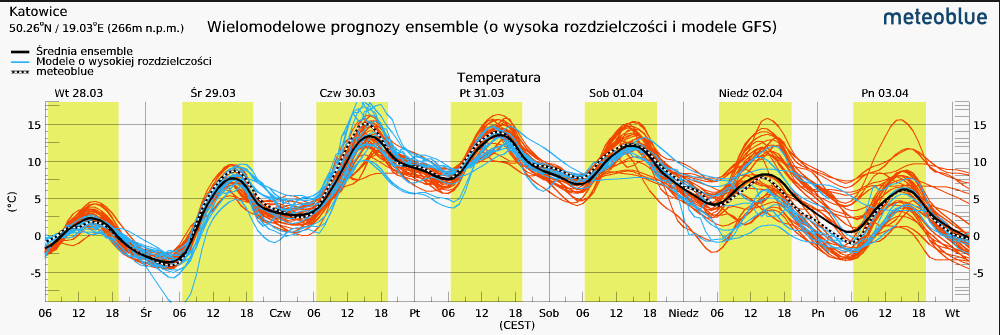
\includegraphics[width=\textwidth]{images/multimodel.png}
    \caption{Przykładowy wynik działania modelu ensemble pochodzący ze strony 
        \url{https://www.meteoblue.com/pl/pogoda/prognoza/multimodel/katowice_polska_3096472}}
    \label{nwp-ensemble}
\end{figure}

Wczesne metody specyfikacji warunków początkowych opierały się na analizie graficznych wykresów 
pogodowych. Następnie różne metody interpolacji danych były zastąpione przez algorytmy
asymilacji danych oparte na teorii sterowania optymalnego. Obliczanie rzeczywistych wartości
opisujących atmosferę może być opisane jako wnioskowane Bayesowskie oparte na wynikach pomiarów
oraz ich niepewnościach. Te obliczenia skoncentrowane na minimalizacji obiektywnej funkcji 
są przeprowadzane w cztero-wymiarowej przestrzeni aby otrzymać fizycznie możliwy wynik
równomiernie rozłożony w trzech wymiarach przestrzennych i czasie.

W praktyce wykorzystanie modeli NWP w celach predykcji pogody wymaga asymilacji dużej ilości
danych pochodzących z różnych źródeł. Metodą wykorzystywaną dzisiaj w celu wprowadzenia
danych jest asymilacja 4D-Var (używana od 1980 roku). W tym algorytmie dla każdego typu obserwacji tworzony jest
operator obserwacji pozwalający wewnętrznym parametrom modelu NWP na odniesienie się
do poszczególnego typu obserwacji. Podczas procesu asymilacji danych parametry wewnętrzne
modelu są dostosowywane aby jak najlepiej odzwierciedlić rzeczywiste warunki pogodowe.

W wielu przypadkach złożoność obliczeniowa NWP wymaga redukcji objętości danych pochodzących
z obserwacji satelitarnych o dużej gęstości. Rozdzielczość danych pochodzących z odczytów
satelitarnych znacznie przekracza możliwości dotychczas używanych modeli stworzonych przez
ECMWF posiadających rozdzielczość horyzontalną równą 9 km. Co więcej w przypadku modeli
ensemble w celach zmniejszenia kosztów obliczeniowych rozdzielczość jest zmniejszana do 18 km.
Procesy które nie mogą być wiernie odzwierciedlone przez symulację
ze wzlędu na zbyt małą rozdzielczość NWP podlegają parametryzacji.
Do takich procesów zalicza się: formowanie się chmur, ilość promieni słonecznych docierających do 
podłoża, opór aerodynamiczny szczytów górskich czy formowanie się kropolek wody.

Ostateczny wynik przeprowadzonej symulacji NWP musi być jeszcze dodatkowo wzbogacony przez zastosowanie
statystyk wyjścia modelu (MOS). W ramach tego prognozowany stan modelu opisywany poprzez skomplikowane
parametry jest zamieniany na wielkości łatwo interpretowalne przez ludzie. Co więcej metody numeryczne
wykorzystują przybliżoną siatkę modelującą atmosferę, która musi być zinterpolowana w celu uzyskania
wyniku dla konkretnej lokalizacji. W tych celach często stosuje się wielokrotne zastosowanie 
regresji liniowej. Krok ten dodatkowo umożliwia zniwelowanie błędów nawarstwionych przez model i wzięcie
pod uwagę sparametryzowanych zjawisk.

Jednym z większych problemów NWP jest nieliniowo wzrastający błąd ograniczający długość prognozy.
Ponieważ modele NWP dokonują predykcji w sposób stopniowy, prognozując stan systemu dla następnego
kroku, żeby później otrzymany wynik dodać do danych wejściowych i kontynuować obliczenia, otrzymane błędy
mają tendencję do akumulacji wraz ze wzrostem długości symulacji.
Limit dla wydarzeń o małej skali jest szacowany na dni, bądź godziny, zaś zdarzenia o dużej skali
mogą być prognozowane z aż 2 tygodniowym wyprzedzeniem. Szacuje się że błąd akumulowany przez 
model NWP ulega zdwukrotnieniu z każdymi pięcioma dniami.

W porównaniu z wieloma innymi dziedzinami w których numeryczne prognozowanie jest stosowane,
NWP ma przewagę pod względem częstotliwości z którą jest wykorzystywane. Prognozy są generowane
w ten sposób z częstotliwością dzienną i na poziomie globalnym. Dokładność tworzonych predykcji jest
dobrze znana i sposoby wzmocnienia aktualnie stosowanych algorytmów mogą być sprawdzone z dużą
efektywnością. Modele NWP wciąż są ulepszane, a rozwój technologiczny i naukowy być może pozwoli
w przyszłości tworzyć modele bazujące na danych zbieranych z rozdzielczością sięgającą 1 km. Co więcej
możliwe że w najbliższej przyszłości utworzone zostaną modele rozwiązujące sprzężone symulacje
dla atmosfery, lądu oraz oceanu\cite{nwp-the-quiet-revolution}.

Dzisiejsze komputery używane do NWP sięgają mocy obliczeniowej równej jednego petaflop-a ($10^{15}$ operacji
zmiennoprzecinkowych) na sekundę. Szacuje się że systemy komputerowe stosowane przez ECMWF mają zużycie energii
sięgające 10 MVA, a dalszy rozwój i zwiększenie modeli mogłoby wymagać 10-krotne zwiększenie pobieranej mocy.


\subsubsection*{Metody uczenia maszynowego}

Problem prognozowania pogody można opisać przy pomocy metody regresji. Polega ona
na statystycznym modelowaniu odpowiedzi nieznanych wartości funkcji na podstawie
znanych wartości zmiennych niezależnych. W ramach przewidywania pogody, za zmienne niezależne
można przyjąć znane wartości pomiarów atmosferycznych i przy pomocy regresji oszacować 
wartości przewidywane. Użyteczne mogą być także metody klasyfikacji w celu wykrywania i 
przewidywania zjawisk pogodowych. W następującej pracy jednak w celu prognozowania pogody
zastosowane będą następujące metody regresji z zakresu uczenia maszynowego:


\begin{itemize}
    \item SVR - jest metodą regresji wykorzystującą maszynę wektorów nośnych w celu tworzenia
    predykcji. Opiera się ona na tworzeniu hiperpłaszczyzny mającej na celu z jak największą
    dokładnością rozdzielenie obserwacji ze zbioru treningowego. Następnie wyznaczone
    równanie hiperpłaszczyzny jest wykorzystywane do klasyfikacji i liczenia regresji dla naukowych
    danych.

    Obliczenie równania hiperpłaszczyzny sprowadza się do problemu optymalizacyjnego
    maksymalizowania odległości hiperpłaszczyzny od punktów należących do poszczególnych klas.
    Ponad przeprowadzanie regresji liniowej, SVR jest w stanie tworzyć regresji nieliniowe
    poprzez zastosowanie "kernel trick", niejawnie mapując dziedzinę danych wejściowych na 
    wielowymiarową przestrzeń o innej charakterystyce.
    
    \item Regresja Logistyczna - jest modelem statstycznym przewidującym nastąpienie danego
    zdarzenia na podstawie obliczenia funkcji logitowej z kombinacji liniowej zmiennych 
    niezależnych.

    \item SGD - jest metodą trenowania modeli uczenia maszynowego poprzez iteratywną optymalizaję
    funkcji celu. Zastosowanie SGD uzyskało dobre wyniki w trenowaniu modeli stosowanych
    do klasyfikacji tekstu i przetwarzaniu języka naturalnego. W ramach tego algorytmu,
    punkt początkowy wybierany przez użytkownika jest poddawany iteratywnej optymalizacji
    poprzez wybieranie kierunku największego spadku funkcji błędu. W ten sposób przestrzeń rozwiązań
    jest przeszukiwana w bardzo efektywny sposób. Niestety zapewnienie globalnego minimum
    nie jest zawsze zagwarantowane.

    \item KNN - jest prostym modelem który może być stosowany zarówno do regresji jak i klasyfikacji.
    Polega na wybraniu k najbliższych sąsiadów ze zbioru treningowego aby określić wartość dla nowej
    obserwacji. Po wybraniu najbardziej podobnych obserwacji ze zbioru treningowego wartość funkcji
    celu jest uśredniana.

    \item Regresja Gaussowska - 
    \item PLS
    \item Drzewo Decyzyjne
    \item Las Losowy
    \item MLP
    \item RNN
    \item CNN
\end{itemize}

% Overview of existing literature: Provide a comprehensive overview of the 
% existing literature on weather prediction and the use of artificial intelligence 
% and machine learning techniques in this area. This could involve summarizing the 
% findings of previous studies, identifying key themes and trends, and highlighting 
% any gaps or limitations in the current literature.
\subsection{Istniejące źródła}

Można znaleźć artykuły analizujące najczęściej występujące słowa
w publikacjach dotyczących algorytmów przewidywania pogody 
\cite{ml-in-weather-prediction}. Okazuje się że w artykułach traktujących o
metodach NWP najczęściej występującą frazą jest "prognozowanie wiatru". Innymi 
często występującymi sformuowaniami były "modele ensemble", "asymilacja danych",
"warunki ekstremalne". Pośród analizowanych artykułów słowo wiatr pojawiło się
ponad 200 razy, najczęściej w odniesieniu do źródeł odnawialnej energii i badań
w przewidywaniu siły wiatru. Słowo opady pojawiło się prawie 150 razy, zazwyczaj
odnosząc się do wykorzystania w prognozowaniu krótkoterminowym, post-processingu, czy
downscaling. 

Z kolei dla artykułów dotyczących uczenia maszynowego
w dziedzinie klimatu najczęściej występujące frazy to "zmiana klimatu", 
"wpływ na klimat", "warunki ekstremalne". Okazuje się że o wiele częstsze było
wystąpienie określenia "globalne modele klimatyczne" niż "regionalne modele 
klimatyczne". 

Wśród istniejących publikacji popularnymi tematami są także korekcja odchylenia 
temperatury i ciśnienia atmosferycznego, analiza promieniowania słonecznego w celach
zasilania instalacji fotowoltaicznych.

\subsubsection*{Wyniki analizowanych źródeł}

\Citeauthor*{machine-learning-for-applied-weather-prediction}
\cite{machine-learning-for-applied-weather-prediction} stworzyli system 
o nazwie DICast podnoszący dokładność modeli numerycznych o 10-15\% przy pomocy
uczenia maszynowego. Zaletą zastosowanego przez nich podejścia jest możliwość
użycia małego zbioru danych do treningu oraz dynamicznej aktualizacji do 
najnowszych informacji.

Badania podsumowane w  przez  \Citeauthor*{ai-revolutionises-weather-prediction}
\cite{ai-revolutionises-weather-prediction}
stwierdzają polepszenie dokładności metod numerycznych ulepszonych przy
pomocy ML w stosunku do bazowych modeli. Odnotowane polepszenie wyników
sięgało 12.4\% dla wilgotności, 5.2\% dla prędkości wiatru, 17.0\% dla
temperatury.

\Citeauthor*{weather-monitoring-using-artificial-intelligence}\cite{weather-monitoring-using-artificial-intelligence}
wybrali regresję liniową do modelowania pogody i zaobserwowali 3.5 procentową
dewiację dla prognozy na następny dzień.

Porównanie wielu modelów, w tym sieci neuronowej, sieci radialnej, 
drzew GBT, regresji liniowej i lasu losowego przez 
\Citeauthor*{developing-machine-learning-algorithms}
\cite{developing-machine-learning-algorithms} wskazuje na 
najlepsze wyniki uzyskiwane przez sieć neuronową. Osiągnęła ona 
współczynnik korelacji równy 84.62\% w zadaniu prognozowania
pogody z miesięcznym wyprzedzeniem. Także \Citeauthor*{weather-forecasting-using-dl} 
\cite{weather-forecasting-using-dl} wskazuje na dobrą dokładność
sieci neuronowych podczas prognozowania opadów.

\Citeauthor*{ml-applied-to-weather-forecasting}
\cite{ml-applied-to-weather-forecasting} wnioskuje że metody 
numeryczne są w stanie osiągnąć lepsze wyniki dla prognoz 
krótkoterminowych, lecz różnica dla prognoz długoterminowych
nie była już tak znaczna. Proponowanym wytłumaczeniem tego jest
brak stabilności modeli NWP i akumulacja błędów dla dłuższych 
okresów czasu. Z kolei uczenie maszynowe zdaje się być bardziej
odporne na perturbacje w warunkach początkowych i zachowuje 
stabilne wyniki nawet dla prognoz długoterminowych.

Mimo wszystko kwestia zastąpienia NWP przez metody uczenia maszynowego
wciąż nie jest roztrzygnięta jak wskazuje \Citeauthor*{can-dl-beat-numerical}
\cite{can-dl-beat-numerical}. Artykuł ten szacuje jakość prognoz 
deterministycznych publikowanych przez ECMWF na 80\% dokładności w przewidywaniu
poziomu ciśnienia na przełomie 7 dni. Z kolei temperatura może być 
prognozowana z błędem średnio-kwadratowym równym 2 stopnie. Wśród wymienionych
zastosowań uczenia głębokiego było szacowanie dystrybucji parametrów przy pomocy 
sieci rekurencyjnej i konwolucyjnej. Innym zastosowaniem było uchwycenie
niepewności z obserwacji w kontekście prognozowania opadów.

Jednym z bardziej wszechstronnych źródeł porównujących aż 24 modele z zakresu
uczenia maszynowego był \Citeauthor*{comparison-of-ml-methods}\cite{comparison-of-ml-methods}.
W tej pracy autor porównywał wybrane modele w celu przewidywania energii fotowoltaicznej
na następny dzień bazując na algorytmach NWP. W tym celu zastosowane było pięć metryk
weryfikacyjnych. Najlepszym modelem w przedstawionym problemie okazała się regresja 
kernel-ridge, wykazująca się także najdłuższym czasem treningu i wysokim zużyciem pamięci.
Algorytmem zalecanym do wykorzystania praktycznego był perceptron wielowarstwowy (MLP)
osiągający zbliżone wyniki do regresji kernel-ridge, lecz wymagający o wiele mniej zasobów.
Co więcej, jednym z wniosków tej pracy jest duże znaczenie wyboru zmiennych w danych wejściowych
na jakość wytrenowanego modelu. Powiększenie danych o dodatkowe informacje przyniosło
wyniki lepsze o 13.1\% w porównaniu do podstawowych zestawów atrybutów. Dalsze polepszenie
mogło być uzyskane poprzez dostrojenie hiperparametrów, umożliwiające zmniejszenie 
RMSE o 3.1\%. Dostosowanie hiperparametrów miało większy wpływ w algorytmach opartych
na drzewach decyzyjnych niż MLP, gradient boosting czy regresji. 

Kolejnym artykułem z tej dziedziny jest \Citeauthor*{coupling-data-science}\cite{coupling-data-science}
analizujący wartość nasłonecznienia. Głównym problemem napotkanym podczas
badań okazało się być znalezienie dobrej równowagi pomiędzy płynnością zmian a 
momentalnymi anomaliami w przewidywanych wartościach. Zastosowanie algorytmów
preferujących ciągłość kończyło się dążeniem prognozy do średniej wartości i 
dużymi błędami podczas zachmurzonych i słonecznych dni. Tak więc dalsza analiza 
wartości odstających i możliwości ich przewidywania jest potrzebna.

\Citeauthor{development-and-application-of-ml-in}\cite{development-and-application-of-ml-in}
zwraca uwagę na potrzebę dostosowania algorytmów AI do problemów związanych z prognozowaniem
pogody. Aspektem branym szczególnie pod uwagę w tej pracy jest wykorzystanie uczenia
maszynowego w celu przewidywania poziomu zanieczyszczeń powietrza. Większość
badań w celu dostosowania algorytmu do swoich danych stosuje dostrajanie hiperparametrów,
preprocessing lub wykorzystywanie modeli ensemble. 

Niektóre analizowane podejścia wykorzystują dość proste algorytmy w celu analizy
problemu. Tak na przykład \Citeauthor{weather-forecast-prediction-data-mining}
\cite{weather-forecast-prediction-data-mining} wykorzystuje drzewa decyzyjne C5 
aby prognozować temperaturę maksymalną, temperaturę minimalną, opady, prędkość wiatru
oraz odparowanie wody. Zastosowany algorytm wykorzystany został w celu tworzenia prognoz
na przekroju miesięcy i lat. Ilustruje to, że nawet proste modele AI są w stanie 
przynieść porządane wyniki, choć niekoniecznie mogące konkurować z dokładnością i 
złożonością algorytmów NWP.

Zastosowanie uczenia maszynowego w celach predykcji pogody znajduje zastosowanie
w sytuacjach w których ilość zasobów obliczeniowych jest ograniczona. Tak więc
\Citeauthor{weather-forecasting-using-ml}\cite{weather-forecasting-using-ml} wykorzystuje
mikrokontrolery przeprowadzające analizę w czasie rzeczywistym bazując na odczytach z 
czujników. Podobnie \Citeauthor{smart-weather-forecasting}\cite{smart-weather-forecasting}
proponuje wykorzystanie internetu rzeczy (IoT) aby zbierać i przetwarzać dane z różnych lokacji.
Dane gromadzone w czasie rzeczywistym mają potencjał rozszerzyć istniejące zbiory danych
i w konsekwencji polepszyć dokładność trenowanych modeli.

W wielu wymienionych pracach \cite{development-and-application-of-ml-in}
były zastosowane różne metryki. Wśród najpopularniejszych
należały RMSE, współczynnik korelacji, MSE, MAE, współczynnik Kappa Cohena,
znormalizowany pierwiastek z błędu średniokwadratowego (NRMSE).

\Citeauthor*{ai-revolutionises-weather-prediction}\cite{ai-revolutionises-weather-prediction}
podkreśla kluczowe zastosowanie uczenia maszynowego w procesie asymilacji danych do modeli NWP.
Jednym z podanych przykładów jest możliwość połączenia zadania pobierania i fuzji danych 
przez jedną sieć neuronową łączącą dane pochodzące ze zdjęć z satelit geostacjonarnych oraz 
pomiarów ilości opadów. Inne przykłady obejmują zastosowanie sieci konwolucyjnych do łączenia
obrazów spektralnych i przestrzennych pochodzących z satelity SEVIRI. 

% Theoretical framework: Identify and discuss any theoretical frameworks that are 
% relevant to your research, and explain how these frameworks have been applied in 
% previous studies.
\subsection{Ramy teoretyczne}

% Methodological approaches: Discuss the different methodological approaches 
% that have been used in previous studies, including the types of data sources used, 
% the modeling techniques employed, and the evaluation metrics used to measure 
% performance.
\subsection{Podejście metodologiczne}

% Critical analysis: Provide a critical analysis of the existing literature, 
% highlighting any strengths or weaknesses in previous studies, and identifying 
% areas where further research is needed.
\subsection{Analiza krytyczna}

% The contribution of your research: Conclude by discussing how your research 
% contributes to the current state of knowledge on weather prediction and the 
% application of artificial intelligence and machine learning techniques in this area. 
% This could involve discussing the novelty of your approach, the potential 
% impact of your findings, or the implications for future research.
\subsection{Wkład pracy}